\newpage
\section{Deliverables}

\subsection{EOM-based optical breadboard setup}

The sponsor already has optical breadboards, as well as a supply of optical equipment which we can use.  We must set up an optical breadboard in a configuration which includes the electro-optic modulator (EOM).

\begin{figure}
  \centering
  \label{setup}
  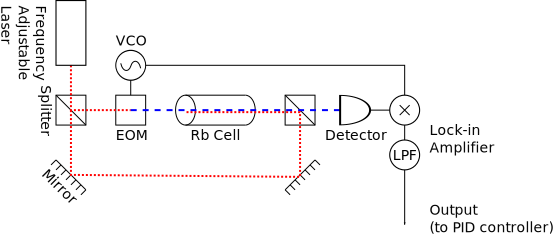
\includegraphics[scale=0.9]{setup.pdf}
  \caption{Overall system setup}
\end{figure}

We must select an appropriate EOM for this purpose which has appropriate characteristics TODO Jeff/Steve we need to pick one to solidify the proposal.

This deliverable should be relatively low-work, as the sponsor already has a working setup, and all that is required is to replicate this setup using an EOM instead of an AOM.

\subsection{Fast Analog Laser Control Feedback Circuit}

Construct an analog feedback circuit to provide an error signal.  The feedback circuit should take advantage of the improved frequency response of the EOM (compared to AOM).  It should have a characteristic response time on the order of 1MHz, as opposed to the 10kHz response time of the existing AOM-based solution.

